Figure~\ref{pgfplot:201306061829} shows the breakdown of the cost for sending UMP messages depending on which cores communicate. The measurement has been executed on ziger1. Propagation time is calculated from the round-trip time minus send and receive time on sender minus processing time on server
\pgfplotsset{width=\linewidth}
\begin{figure}
  \caption{UMP breakdown}
  \label{pgfplot:201306061829}
  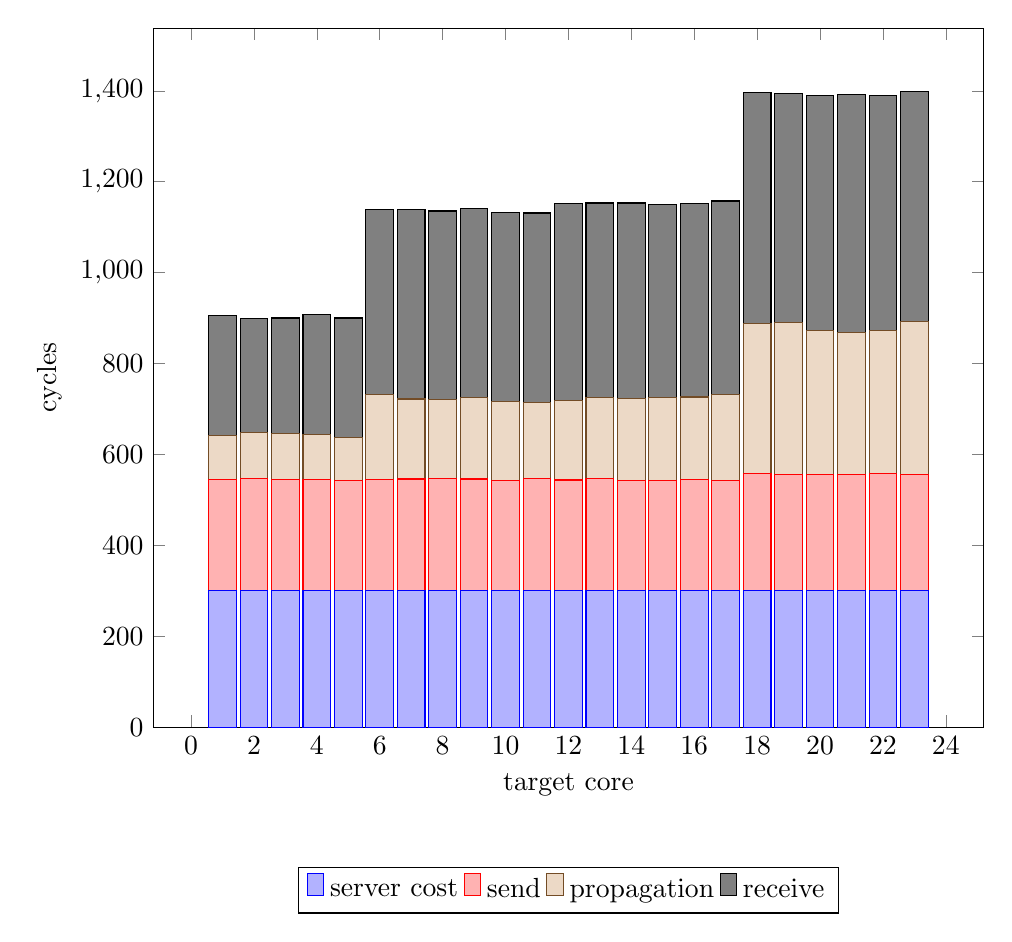
\begin{tikzpicture}
    \begin{axis}[
        ybar stacked,ymin=0,legend style={ at={(0.5,-0.20)}, anchor=north, legend columns=-1},
        xlabel={target core},
        ylabel={cycles}
        ]
    \addplot coordinates {
      (1,300.000000)
      (2,300.000000)
      (3,300.000000)
      (4,300.000000)
      (5,300.000000)
      (6,300.000000)
      (7,300.000000)
      (8,300.000000)
      (9,300.000000)
      (10,300.000000)
      (11,300.000000)
      (12,300.000000)
      (13,300.000000)
      (14,300.000000)
      (15,300.000000)
      (16,300.000000)
      (17,300.000000)
      (18,300.000000)
      (19,300.000000)
      (20,300.000000)
      (21,300.000000)
      (22,300.000000)
      (23,300.000000)
    };
    \addplot coordinates {
      (1,244.197531)
      (2,246.407407)
      (3,245.567901)
      (4,244.543210)
      (5,243.530864)
      (6,245.061728)
      (7,245.901235)
      (8,247.481481)
      (9,245.901235)
      (10,243.197531)
      (11,246.530864)
      (12,243.913580)
      (13,246.259259)
      (14,243.469136)
      (15,242.283951)
      (16,244.851852)
      (17,242.209877)
      (18,258.012346)
      (19,256.765432)
      (20,256.592593)
      (21,255.382716)
      (22,258.666667)
      (23,255.567901)
    };
    \addplot coordinates {
      (1,98.388889)
      (2,102.181481)
      (3,101.376543)
      (4,99.783951)
      (5,93.748148)
      (6,187.491358)
      (7,176.212346)
      (8,173.327160)
      (9,178.597531)
      (10,173.375309)
      (11,167.481481)
      (12,175.728395)
      (13,179.177778)
      (14,180.565432)
      (15,183.571605)
      (16,181.665432)
      (17,189.946914)
      (18,331.055556)
      (19,333.632099)
      (20,315.514815)
      (21,313.348148)
      (22,314.414815)
      (23,337.682716)
    };
    \addplot coordinates {
      (1,262.716049)
      (2,250.864198)
      (3,253.271605)
      (4,264.481481)
      (5,262.876543)
      (6,406.592593)
      (7,417.086420)
      (8,414.913580)
      (9,417.024691)
      (10,416.345679)
      (11,417.320988)
      (12,432.172840)
      (13,427.814815)
      (14,429.234568)
      (15,424.814815)
      (16,426.283951)
      (17,425.444444)
      (18,506.333333)
      (19,503.679012)
      (20,518.222222)
      (21,522.506173)
      (22,517.111111)
      (23,504.703704)
    };
     \legend{server cost, send, propagation, receive}
    \end{axis}
  \end{tikzpicture}
\end{figure}
